\section{Local Imitation Dynamics for Public Good Games}
\subsection{Outline}
This chapter investigates the linear PGG under imitation dynamics. Imitation dynamics are introduced in equation \eqref{rep}, with $\alpha = 0$. Given $\pi_j>\pi_i$, the transition probability $q_{i\to j} = 1$. The tests from Chapter \ref{Chapter:Rep} are run for imitation dynamics, and the similarities and differences to replicator dynamics are noted. In general, imitation dynamics induces less contribution than replicator dynamics. The greatest difference is noticed for RRG models, as they fail to achieve non-zero contribution. The positive correlation between degree size variance and contribution mirrors the results in Chapter \ref{Chapter:Rep}. 

\subsection{Results}
\FloatBarrier
\graphCap{ID_gtype_low.pdf}{0.7}{Comparing graph models: imitation dynamics. Trend for $r \in \{4.0, 4.25, 4.5, 4.75\}$. In each graph, the blue circles, orange stars, green crosses, and red pentagons correspond to the WS model, TAG model, BA model, and RRG model respectively. Only the BA graph model induces non-trivial contribution.}{imitation_low} 
\FloatBarrier
\graphCap{ID_gtype_med.pdf}{0.7}{Comparing graph models: imitation dynamics. Trend for $r \in \{5.0, 5.25, 5.5, 5.75\}$. In each graph, the blue circles, orange stars, green crosses, and red pentagons correspond to the WS model, TAG model, BA model, and RRG model respectively. The BA model still induces the highest contribution, and the RRG consistently induces the lowest.}{imitation_medium}
\FloatBarrier
\graphCap{ID_gtype_high.pdf}{0.7}{Comparing graph models: imitation dynamics. Trend for $r \in \{6,6.5,7,7.5\}$. In each graph, the blue circles, orange stars, green crosses, and red pentagons correspond to the WS model, TAG model, BA model, and RRG model respectively. The TAG model overtakes the BA model, while the RRG still fails to achieve non-zero contribution. }{imitation_high}\FloatBarrier

Relative to replicator dynamics, less contribution is observed for each graph model and parameter $r$. Furthermore, the \emph{re-ordering} effect noticed in Figure \ref{replicator_medium} and Figure \ref{replicator_high}, whereby the contribution initially drops and then returns, is not observed to the same level. \\

For $r<6.25$, the order of the models, from most to least contribution, is the BA model, then TAG, then WS, and finally the RRG. In fact, for $r<7$, the RRG model never achieves non-zero contribution. A possible explanation is the faster switching rate of strategies. Under imitation dynamics, player $i$ randomly chooses a neighbour $j$, and then always switches if $\pi_j>\pi_i$. In comparison, under replicator dynamics, the probability of switching is proportional to the difference in payoff. Therefore $i$ does not always switch to $j$, even if $\pi_j>\pi_i$. For this reason, the environment may be able to \emph{re-order}, and spread contribution further before contribution becomes extinct. \\

In the regime $r\geq 6.25$, the TAG model overtakes the BA model for higher contribution. This phenomenon was also noticed under replicator dynamics in Figure \ref{replicator_medium}, but instead occurred at $r=5.25$. A possible explanation is the higher clustering coefficient for the TAG model. This allows groups of contribution to form, which then spread further and induce higher contribution. \\

For consistency, the same tests from Chapter \ref{Chapter:Rep} are reproduced under imitation dynamics. 

\subsection{Isolating the Effect of Clustering Coefficient: Power Law Degree Size Distribution}

\FloatBarrier
\graphCap{ID_power_p_low.pdf}{0.7}{Effect of clustering $p$, PL Model, imitation dynamics. In each graph, the blue circles, orange stars, green crosses, red pentagons, and purple squares correspond to $p\in\{0.1,0.2,0.3,0.4,0.5\}$ respectively. The observed trend is that higher $p$, and hence higher $C_\Delta$, leads to  higher contribution.}{ID_power_p_low}
\FloatBarrier
\graphCap{ID_power_p_med.pdf}{0.7}{Effect of clustering $p$, PL Model, imitation dynamics. In each graph, the blue circles, orange stars, green crosses, red pentagons, and purple squares correspond to $p \in \{0.1,0.2,0.3,0.4,0.5\}$ respectively. The trend is also observed here, with some minor discrepancies. For example, $p=0.4$ induces higher contribution in a $r=5$ regime than $p=0.5$.}{ID_power_p_med} \FloatBarrier

The trend from Figure \ref{power_p_med} is reproduced here, namely that higher $p$, and hence higher $C_\Delta$, induces higher contribution. This could be due to the higher clustering coefficient, or higher degree variance. Also note that the time to stability is much faster in these models than Figures \ref{power_p_low} and \ref{power_p_med}. This is because the probability of agent $i$ adopting agent $j$'s strategy, given $\pi_j > \pi_i$ is always 1 under imitation dynamics. Under replicator dynamics, this is not guaranteed and hence the rate at which strategies are changed is slower. 


\subsection{Isolating the Effect of Clustering Coefficient: Constant Degree Size Distribution}

\graphCap{ID_graph_p_med.pdf}{0.7}{Effect of rewiring $p$, WS model. In each graph, the blue circles, orange stars, green crosses, red pentagons, and purple squares correspond to $p \in \{0.1,0.2,0.3,0.4,0.5\}$ respectively. The trend indicates that higher $p$, and hence lower $C_\Delta$, leads to higher contribution. }{ID_graph_p_med}\FloatBarrier
 


\graphCap{ID_graph_p_high.pdf}{0.7}{Effect of rewiring $p$, WS model. In each graph, the blue circles, orange stars, green crosses, red pentagons, and purple squares correspond to $p \in \{0.1,0.2,0.3,0.4,0.5\}$ respectively. The observed trend is an increase in $p$, and hence a reduction in $C_\Delta$, leads to higher contribution.}{ID_graph_p_high}
\FloatBarrier

 Similar to Figure \ref{graph_p_med}, the effect of high $p$ does not dominate until $r$ is past a certain threshold. The threshold is $5.75$ for replicator dynamics, and $6$ for imitation dynamics. This indicates the impediment to the spread of contribution in a low $r$, high $p$ environment is not unique to replicator dynamics. \\
 
 In general, the trend observed in Figures \ref{graph_p_med} and \ref{graph_p_high} were replicated here. Higher variance in degree distribution leads to higher contribution. However the time to equilibrium is much faster for imitation dynamics.
 
\subsection{The Effect of Mean Degree: RRG}

\graphCap{ID_graph_m_low_RRG.pdf}{0.8}{Effect of mean degree, RRG model. In each graph, the blue circles, orange stars, green crosses, red pentagons, and purple squares correspond to the mean degree $m \in \{4,6,8,10,12\}$ respectively. An increase in $m$ results in lower mean contribution.  }{ID_graph_m_low} \FloatBarrier

\graphCap{ID_graph_m_med_RRG.pdf}{0.8}{Effect of mean degree, RRG model. In each graph, the blue circles, orange stars, green crosses, red pentagons, and purple squares correspond to the mean degree $m \in \{4,6,8,10,12\}$ respectively. An increase in $m$ results in lower mean contribution.  }{ID_graph_m_med} \FloatBarrier



\graphCap{ID_graph_m_high_RRG.pdf}{0.8}{Effect of mean degree, RRG model. In each graph, the blue circles, orange stars, green crosses, red pentagons, and purple squares correspond to mean degree $m \in  \{4,6,8,10,12\}$ respectively. Once again, an increase in $m$ results in lower contribution. }{ID_graph_m_high} \FloatBarrier

It is evident that $r>m+1$ is required for full contribution in the RRG model. It is also interesting  to contrast the trends corresponding to $m=4, r \to 5$, and $m=6, r \to 7$. As $r$ approaches $m+1$ for $m=4$, moderate contribution is induced, however in the case $m=6$, all trials result in a full defection equilibrium. On the other hand, for $m = 6, r \to 7$ in Figure \ref{graph_m_med} and Figure \ref{graph_m_high}, some moderate contribution is observed. This is a major difference between replicator and imitation dynamics. For certainty, the experiment corresponding to $r=7, m =6$ was run and contribution achieved, however it is not reproduced here. 



\subsection{The Effect of Mean Degree: BA Model}
\FloatBarrier
\graphCap{ID_graph_m_low_BA.pdf}{0.8}{Effect of mean degree, BA model. In each graph, the blue circles, orange stars, green crosses, red pentagons, and purple squares correspond to targeted mean degree $m = \{4,6,8,10,12\}$ respectively. For the BA model, an increase in $m$ also results in lower contribution.}{ID_BA_graph_m_low}
\FloatBarrier
\graphCap{ID_graph_m_med_BA.pdf}{0.8}{Effect of mean degree, BA model. In each graph, the blue circles, orange stars, green crosses, red pentagons, and purple squares correspond to targeted mean degree $m = \{4,6,8,10,12\}$ respectively. For the BA model, an increase in $m$ results in lower contribution.}{ID_BA_graph_m_med}
\FloatBarrier

\graphCap{ID_graph_m_high_BA.pdf}{0.8}{Effect of mean degree, BA model. In each graph, the blue circles, orange stars, green crosses, red pentagons, and purple squares correspond to targeted mean degree $m = \{4,6,8,10,12\}$ respectively. For the BA model, an increase in $m$ results in lower contribution.}{ID_BA_graph_m_high}
\FloatBarrier

Firstly, note that the BA model generally reports higher contribution than the RRG model for given $r,m$. This corresponds to previous trials. Under the BA model, some medium levels of contribution are observed. This can be attributed to some realisations of the network inducing full contribution. It is not shown, but the 2.5\% and 97.5\% quantiles were investigated for the BA and RRG models. In the case corresponding to $m=8, r = 4.25$, the 97.5\% quantile BA model was able to achieve full contribution. This contrasts with $m=6, r = 6.75$, where the 97.5\% quantile realisation resulted in no contribution for the RRG model. The variance between realisations of a BA network is much higher, and this leads to reported average equilibria between 0 and 1. 

\subsection{Contribution Level Within a Single Graph Instance: BA model } 
Now the contribution proportion at equilibrium is stratified by degree size, and plotted. Degree sizes with a count less than 6 occurrences are not shown, as they are too easy. This process is called trimming the graph. \\

\FloatBarrier 
\begin{figure}[!h]
  \begin{subfigure}[b]{0.45\textwidth}
    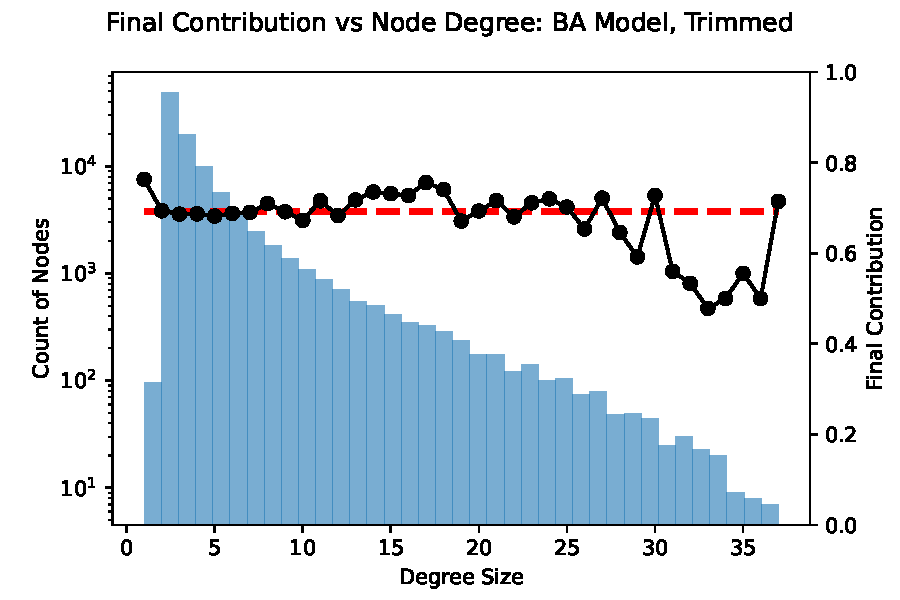
\includegraphics[width=1.1\textwidth]{images/ID_BA_node_groups_m_4_phi_4_trimmed.pdf}
    \caption{Final contribution by degree, BA Model, trimmed, for $m=4$, $r=4$.   }
    \label{ID_by_degree_m_4_phi_4}
  \end{subfigure}
  \hfill
  \begin{subfigure}[b]{0.45\textwidth}
    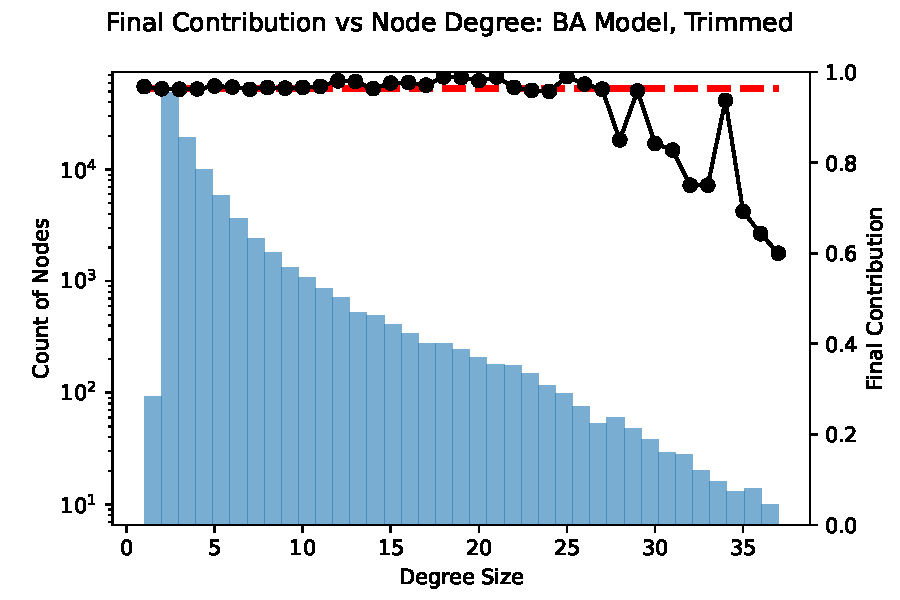
\includegraphics[width=1.1\textwidth]{images/ID_BA_node_groups_m_4_phi_6_trimmed.pdf}
    \caption{Final contribution by degree, BA Model, trimmed, for $m=4$, $r=6$. }
    \label{ID_by_degree_m_4_phi_6}
  \end{subfigure}
  \caption{The histogram, plotted on the left axis, shows the count of nodes with given degree. The black trend line is the mean contribution for nodes of that degree, measured at the final step. Finally, the red line is the overall mean contribution, also measured at the final step. Both plots indicate that higher node degrees contribute less than lower node degrees.} \label{ID_by_degree_m_4}
\end{figure} 
\FloatBarrier


\FloatBarrier 
\begin{figure}[!h]
  \begin{subfigure}[b]{0.45\textwidth}
    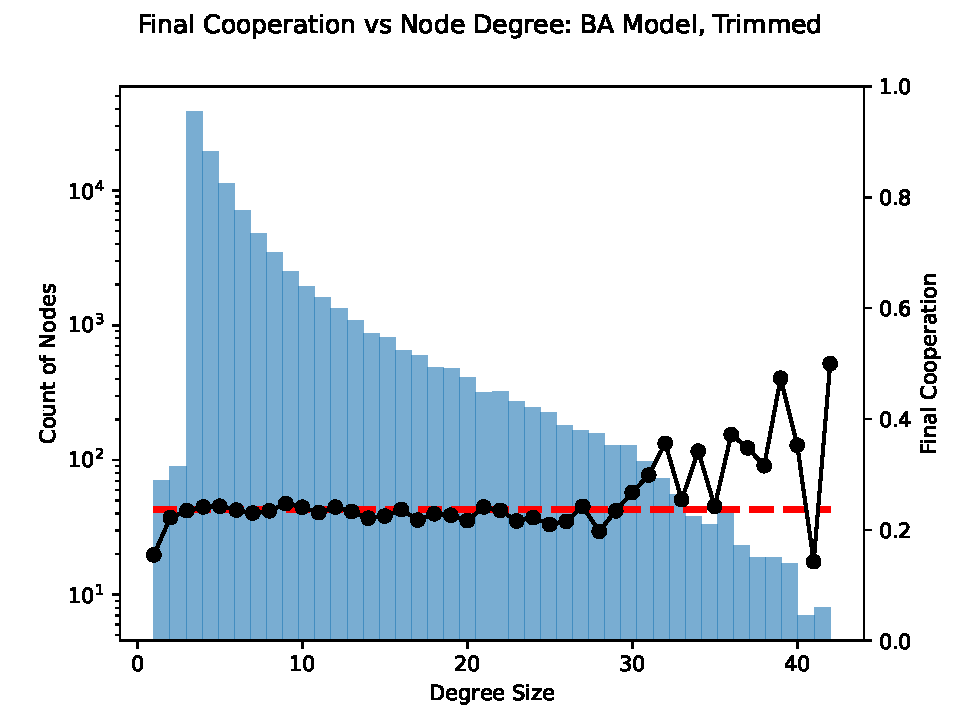
\includegraphics[width=1.1\textwidth]{images/Rep_BA_node_groups_m_6_phi_4_trimmed.pdf}
    \caption{Final contribution by degree, BA Model, trimmed, for $m=6$, $r=4$.   }
    \label{ID_by_degree_m_6_phi_4}
  \end{subfigure}
  \hfill
  \begin{subfigure}[b]{0.45\textwidth}
    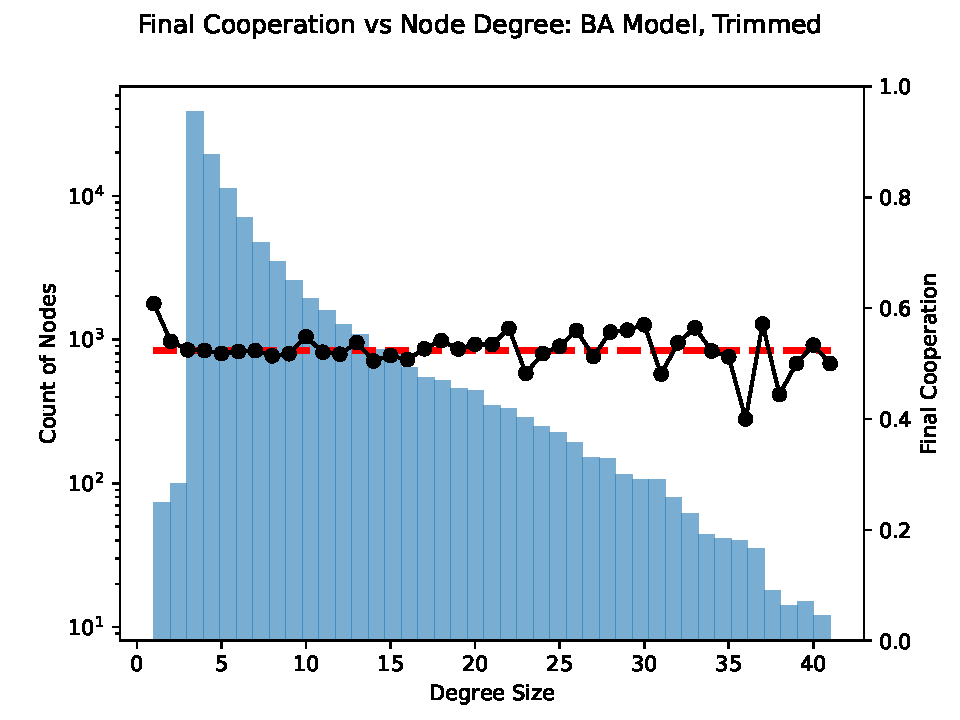
\includegraphics[width=1.1\textwidth]{images/ID_BA_node_groups_m_6_phi_6_trimmed.pdf}
    \caption{Final contribution by degree, BA Model, trimmed, for $m=6$, $r=6$. }
    \label{ID_by_degree_m_6_phi_6}
  \end{subfigure}
  \caption{The histogram, plotted on the left axis, shows the count of nodes with given degree. The black trend line is the mean contribution for nodes of that degree, measured at the final step. Finally, the red line is the overall mean contribution, also measured at the final step. Higher degree nodes contribute more than average in Figure \ref{ID_by_degree_m_6_phi_4}, and similar to average for Figure \ref{ID_by_degree_m_6_phi_6}. } \label{ID_by_degree_m_6}
\end{figure} 
\FloatBarrier


\FloatBarrier 
\begin{figure}[!h]
  \begin{subfigure}[b]{0.45\textwidth}
    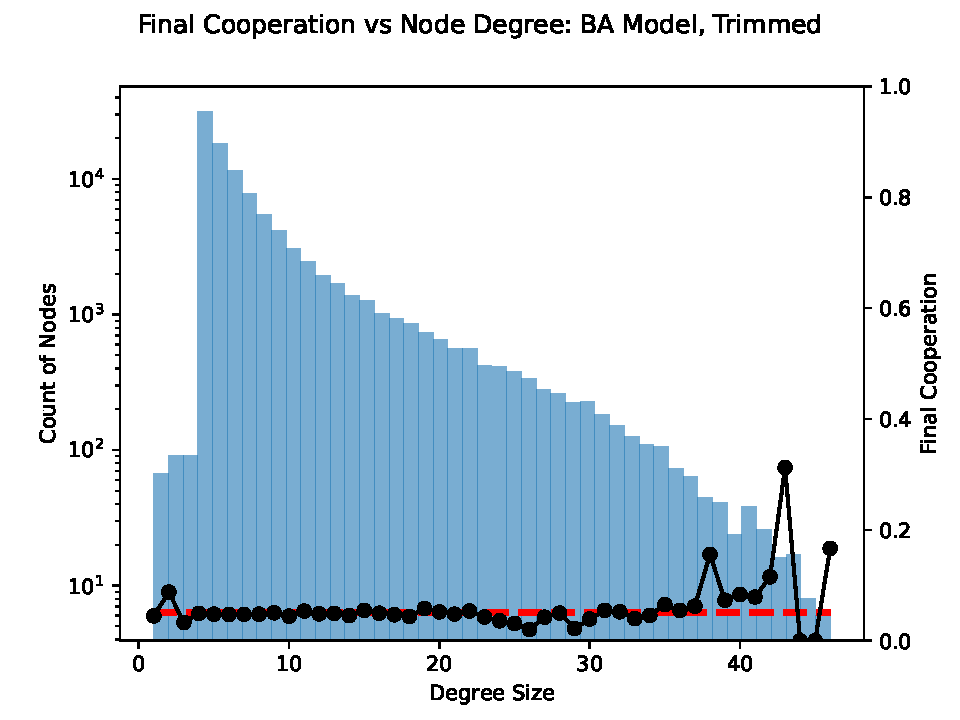
\includegraphics[width=1.1\textwidth]{images/Rep_BA_node_groups_m_8_phi_4_trimmed.pdf}
    \caption{Final contribution by degree, BA Model, trimmed, for $m=8$, $r=4$.   }
    \label{ID_by_degree_m_8_phi_4}
  \end{subfigure}
  \hfill
  \begin{subfigure}[b]{0.45\textwidth}
    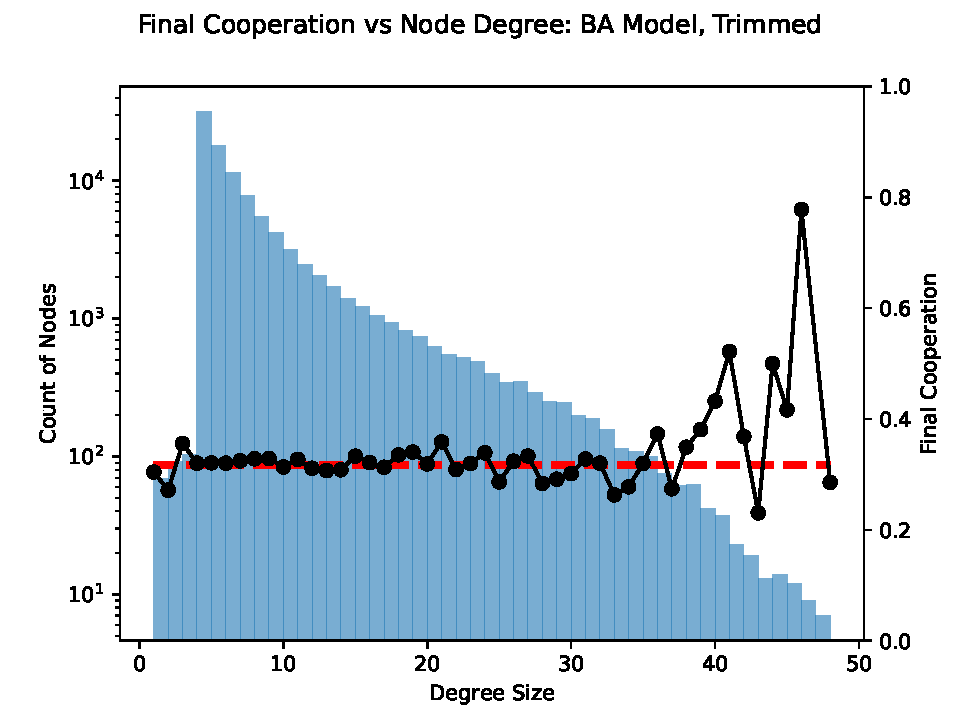
\includegraphics[width=1.1\textwidth]{images/Rep_BA_node_groups_m_8_phi_6_trimmed.pdf}
    \caption{Final contribution by degree, BA Model, trimmed, for $m=8$, $r=6$. }
    \label{ID_by_degree_m_8_phi_6}
  \end{subfigure}
  \caption{The histogram, plotted on the left axis, shows the count of nodes with given degree. The black trend line is the mean contribution for nodes of that degree, measured at the final step. Finally, the red line is the overall mean contribution, also measured at the final step. Both plots indicate that higher node degrees contribute more than lower node degrees.} \label{ID_by_degree_m_8}
\end{figure} 
\FloatBarrier

The trend in these graphs is very similar to that observed in Figure \ref{by_degree_m_4}, Figure \ref{by_degree_m_6}, and Figure \ref{by_degree_m_8}. The nodes with high degree are not as influenced as the low degree nodes, so contribute less in a high contribution environment and more in a low contribution environment. The low degree nodes induce conformity.

\section{Comparison of Replicator and Imitation Dynamics}

Both replicator and imitation dynamics produced a similar ranking of graph models. The graph models with a power-law degree distribution, specifically the BA and TAG models, induced higher contribution than the RRG and WS models. \\

The RRG model never achieved non-zero contribution under imitation dynamics, yet surpassed the WS model and achieved quite substantial contribution under replicator dynamics. This is one of the major differences. \\

Another major difference is the level of maximum contribution achieved. Two figures are replicated below, and show the contribution level, as well as a $95\%$ confidence interval around the mean. \\

\FloatBarrier 
\begin{figure}[!h]
  \begin{subfigure}[b]{0.45\textwidth}
    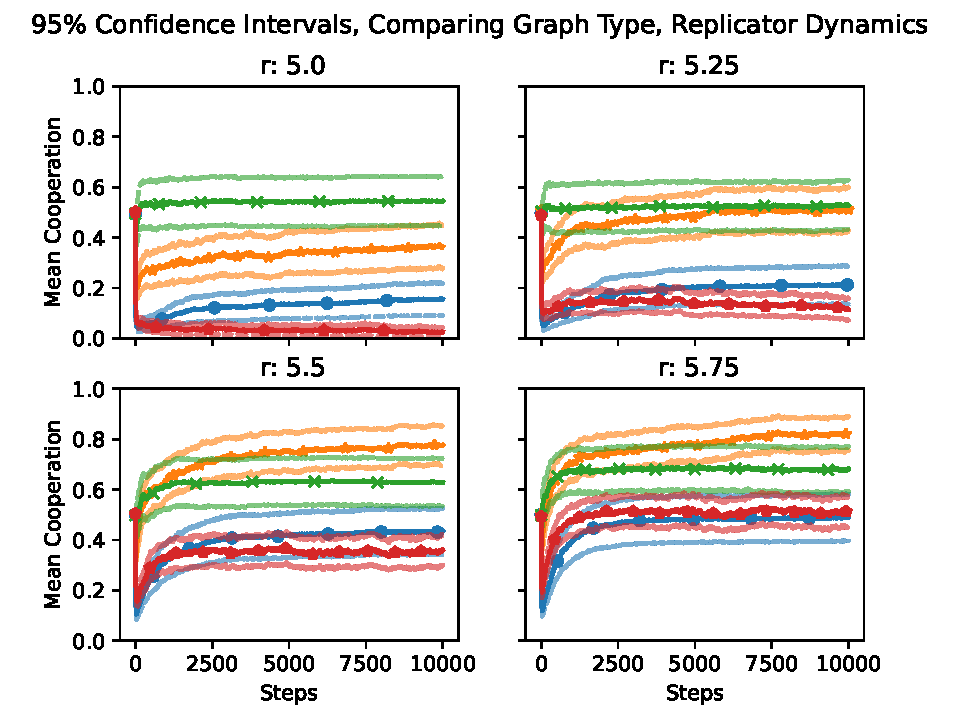
\includegraphics[width=1.1\textwidth]{images/Rep_gtype_med_CI.pdf}
    \caption{Comparing graph models, replicator dynamics.   }
    \label{rep_high_gtype_2}
  \end{subfigure}
  \hfill
  \begin{subfigure}[b]{0.45\textwidth}
    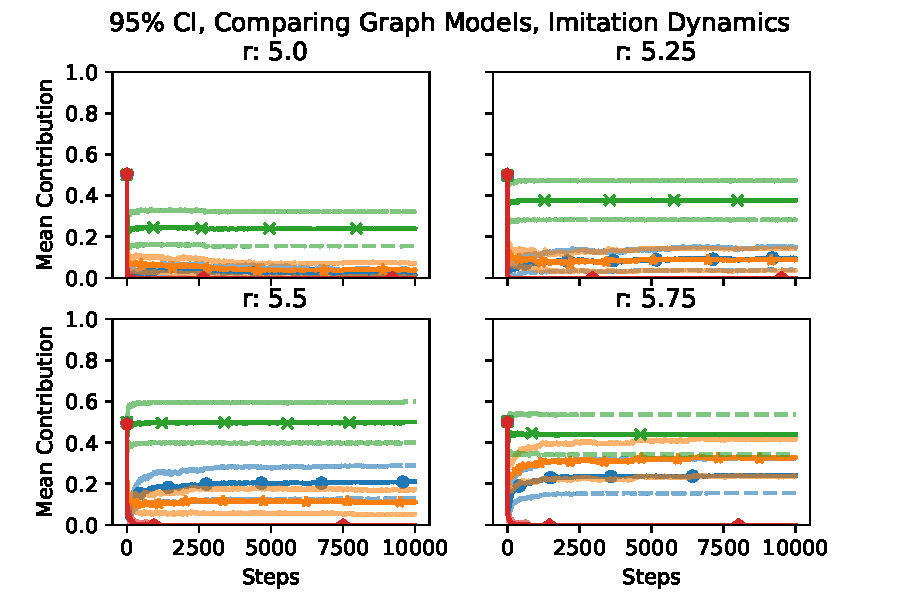
\includegraphics[width=1.1\textwidth]{images/ID_gtype_med_CI.pdf}
    \caption{Comparing graph models, imitation dynamics. }
    \label{ID_high_gtype_2}
  \end{subfigure}
  \caption{Replication of Figure  \ref{replicator_medium} and Figure \ref{imitation_medium} with confidence intervals. For every graph model, replicator dynamics induce higher contribution. The width of the confidence intervals is quite similar between replicator and imitation dynamics. } \label{comparing_rep_ID_high}
\end{figure} 
\FloatBarrier

\begin{comment}
It is hard to examine the size of the confidence intervals visually, so Figure \ref{rep_dev} and \ref{id_dev} collate the standard deviation of contribution in the final timestep for each graph model. \\
\FloatBarrier
\graphCap{Rep_dev_heatmap.pdf}{0.7}{Sample Standard Deviation at the Final Generation, Replicator Dynamics.}{rep_dev}
\FloatBarrier
\graphCap{ID_dev_heatmap.pdf}{0.7}{Sample Standard Deviation at the Final Generation, Imitation Dynamics. }{id_dev}
\FloatBarrier
When comparing Figure \ref{rep_dev} and \ref{id_dev}, it is important to compare the sample standard deviation amongst models that result in the same equilibrium contribution, as opposed to the same $r$ value. For example, the BA model achieves around 0.6 contribution for $r=5.5$ under replicator dynamics, but requires $r=6.5$ for imitation dynamics. At these levels, the sample standard deviation is similar for replicator (0.48) and imitation (0.45) dynamics. A major trend to observe is the difference in sample variance for BA and RRG models under replicator dynamics, even though they attain the same equilibrium values for $6.0\leq r \leq 6.5$. This can be explained by the higher variance in degree distribution for the BA model, which results in vastly different final equilibria. \\
\end{comment}
It is hard to examine the size of the confidence intervals visually, so another measurement is required. It is more explanatory to examine the nature of each realisation of the graph model in the final timestep. To do this, the contribution level of each trial was recorded for each graph model, $r$, and evolution model combination, and plotted on a histogram.

\FloatBarrier 
\begin{figure}[!h]
  \begin{subfigure}[b]{0.45\textwidth}
    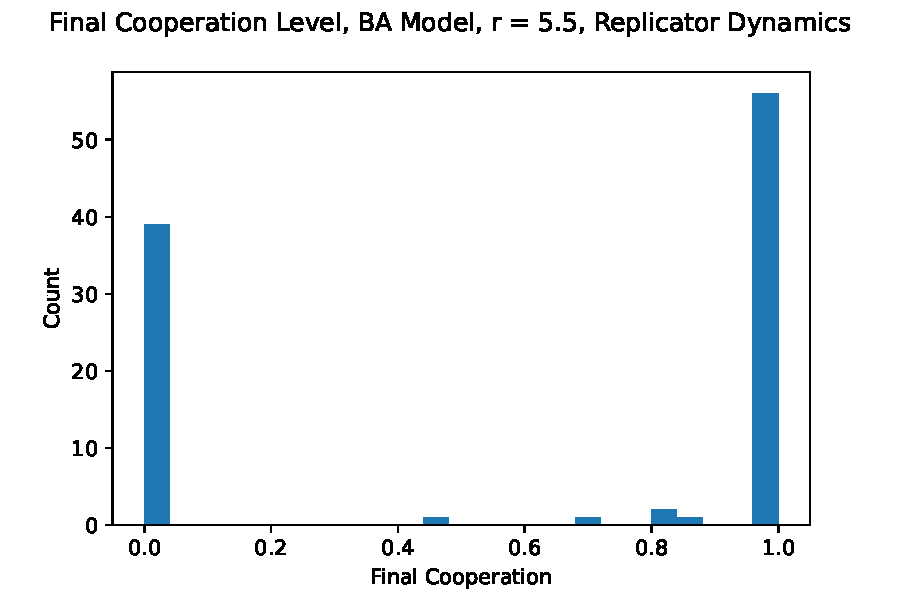
\includegraphics[width=1.1\textwidth]{images/Rep_coop_histo_BA_55.pdf}
    \caption{Replicator dynamics.}
    \label{Rep_BA_55_coop_histo}
  \end{subfigure}
  \hfill
  \begin{subfigure}[b]{0.45\textwidth}
    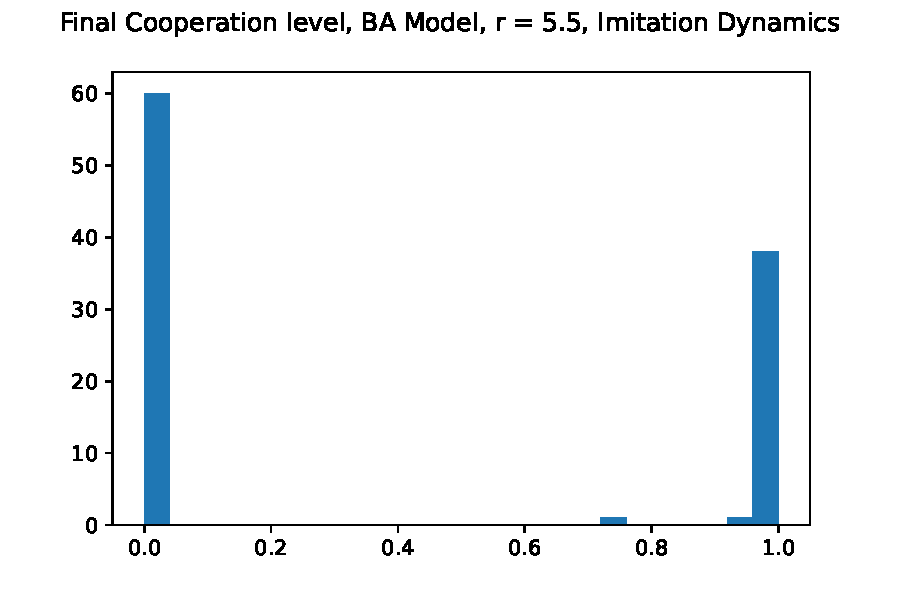
\includegraphics[width=1.1\textwidth]{images/ID_coop_histo_BA_55.pdf}
    \caption{imitation Dynamics. }
    \label{ID_BA_55_coop_histo}
  \end{subfigure}
  \caption{Final contribution level, BA model, $r = 5.5$, replicator and imitation dynamics. } \label{coop_histo_BA}
\end{figure} 
\FloatBarrier

\FloatBarrier 
\begin{figure}[!h]
  \begin{subfigure}[b]{0.45\textwidth}
    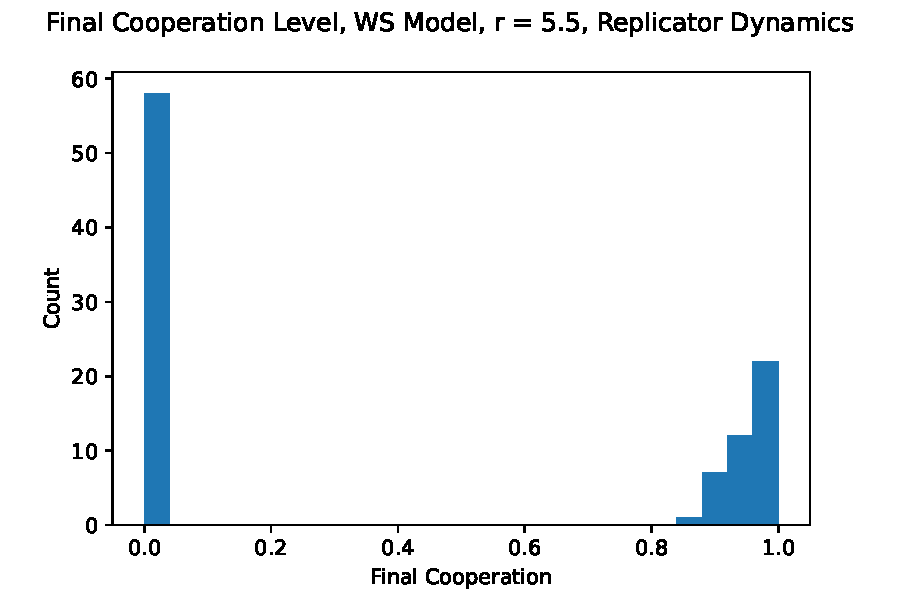
\includegraphics[width=1.1\textwidth]{images/Rep_coop_histo_WS_55.pdf}
    \caption{Replicator dynamics. }
    \label{Rep_WS_55_coop_histo}
  \end{subfigure}
  \hfill
  \begin{subfigure}[b]{0.45\textwidth}
    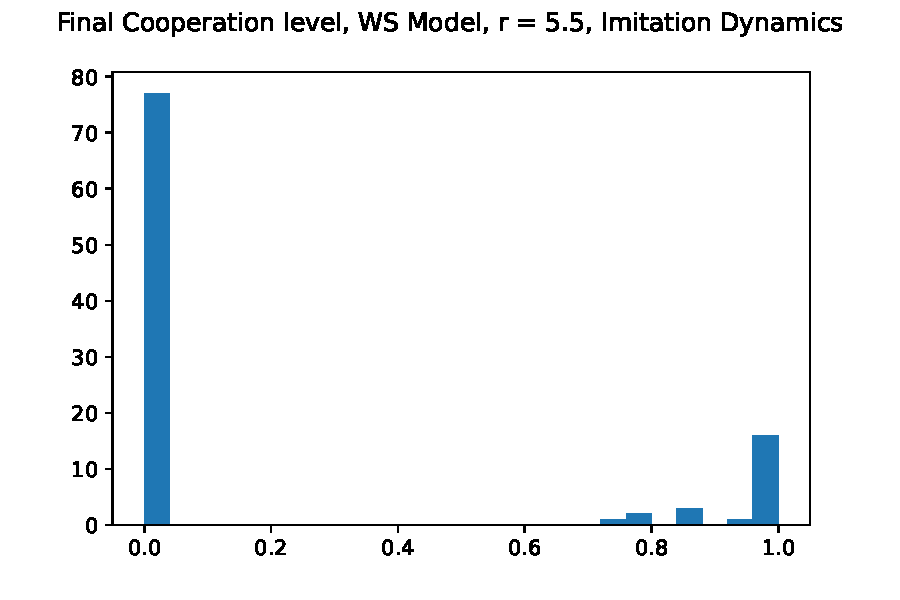
\includegraphics[width=1.1\textwidth]{images/ID_coop_histo_WS_55.pdf}
    \caption{Imitation dynamics. }
    \label{ID_WS_55_coop_histo}
  \end{subfigure}
  \caption{Final contribution level, WS model, $r = 5.5$, replicator and imitation dynamics. } \label{coop_histo_WS}
\end{figure} 
\FloatBarrier

\FloatBarrier 
\begin{figure}[!h]
  \begin{subfigure}[b]{0.45\textwidth}
    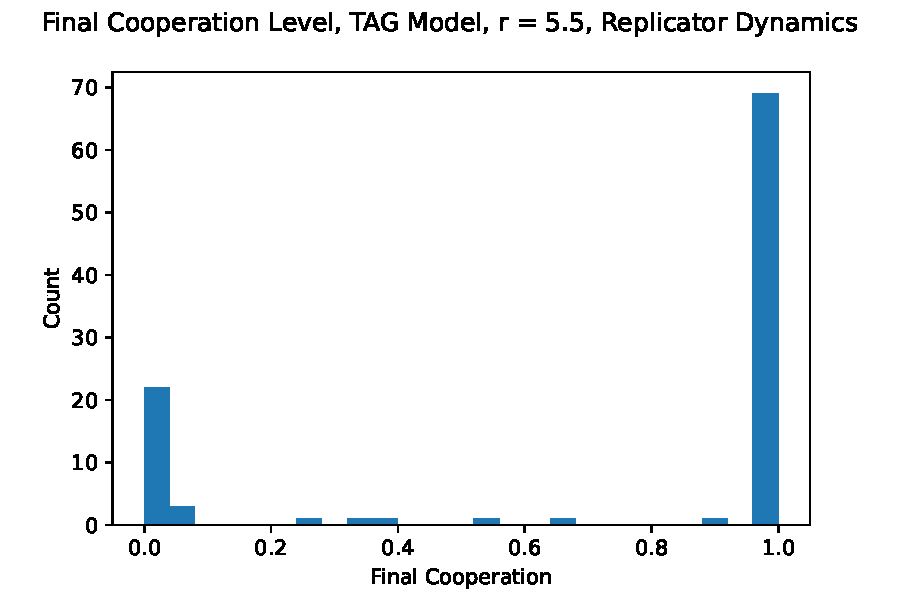
\includegraphics[width=1.1\textwidth]{images/Rep_coop_histo_TAG_55.pdf}
    \caption{Replicator dynamics. }
    \label{Rep_TAG_55_coop_histo}
  \end{subfigure}
  \hfill
  \begin{subfigure}[b]{0.45\textwidth}
    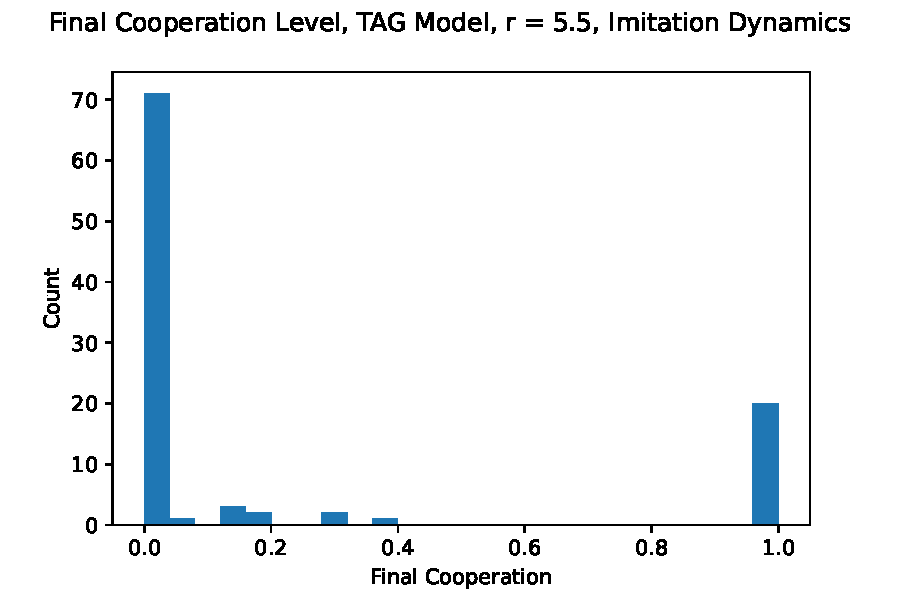
\includegraphics[width=1.1\textwidth]{images/ID_coop_histo_TAG_55.pdf}
    \caption{Imitation dynamics. }
    \label{ID_TAG_55_coop_histo}
  \end{subfigure}
  \caption{Final contribution level, TAG model, r = 5.5, replicator and imitation dynamics. } \label{coop_histo_TAG}
\end{figure} 
\FloatBarrier

\FloatBarrier 
\begin{figure}[!h]
  \begin{subfigure}[b]{0.45\textwidth}
    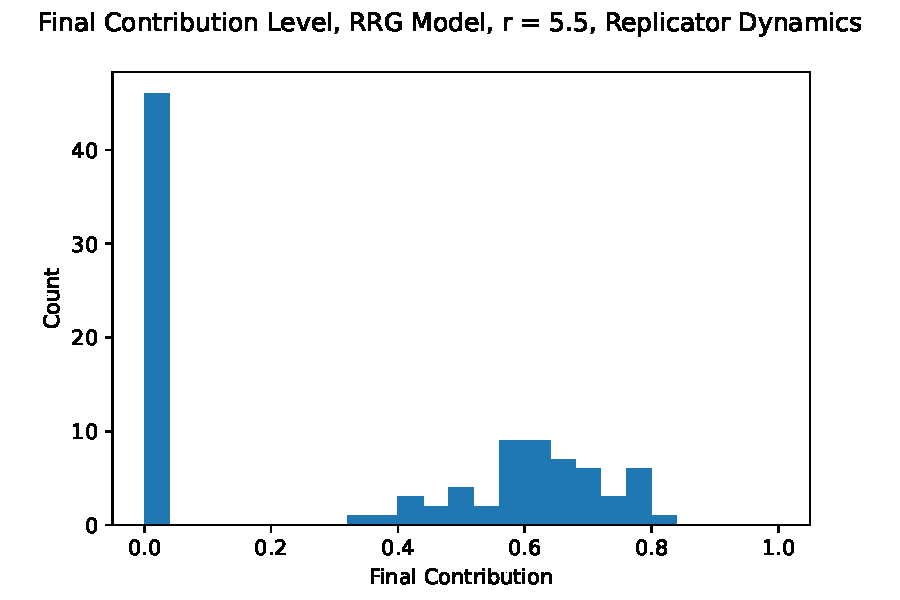
\includegraphics[width=1.1\textwidth]{images/Rep_coop_histo_RRG_55.pdf}
    \caption{Replicator dynamics. }
    \label{Rep_RRG_55_coop_histo}
  \end{subfigure}
  \hfill
  \begin{subfigure}[b]{0.45\textwidth}
    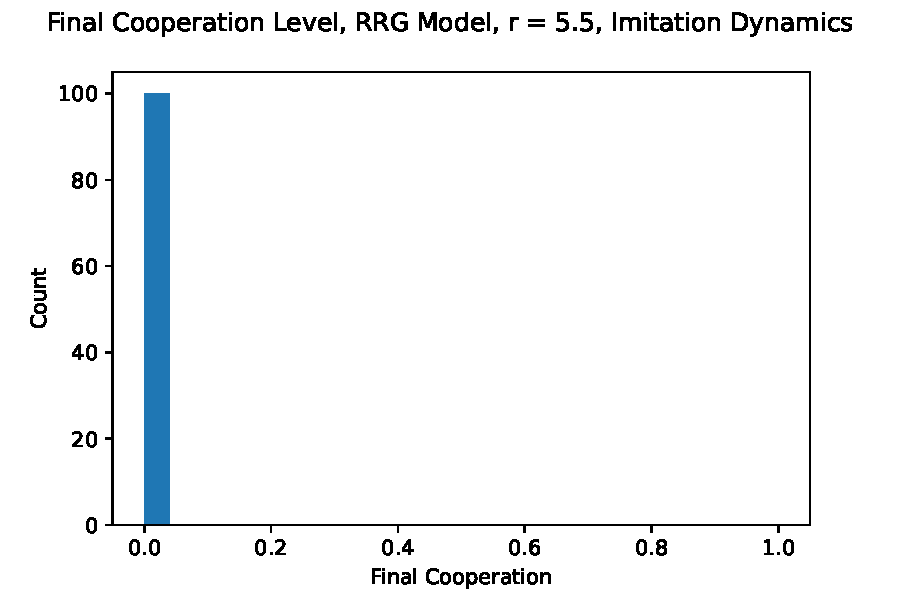
\includegraphics[width=1.1\textwidth]{images/ID_coop_histo_RRG_55.pdf}
    \caption{Imitation dynamics. }
    \label{ID_RRG_55_coop_histo}
  \end{subfigure}
  \caption{Final contribution level, RRG model, $r = 5.5$, replicator and imitation dynamics. } \label{coop_histo_RRG}
\end{figure} 
\FloatBarrier
 It is interesting that replicator dynamics allows for non-extreme equilibrium values, whereas imitation dynamics almost exclusively forces the contribution level to 0 or 1. A possible hypothesis is that the non-extreme values are not in fact equilibria, and are still evolving. If it were the case, one could expect a trail of results approaching the extreme value, whereas in Figure \ref{coop_histo_RRG} the non-zero equilibria are centered around 0.6, and there is quite a range of non-extreme values. This lends credence to the claim that these non-extreme values are in fact equilibria. \\
 



Another difference between replicator and imitation dynamics is the time to equilibrium, particularly in the case where the equilibrium is low contribution. The time to equilibrium in a complete graph model is discussed in Lemma \ref{connected}, and it is shown that replicator dynamics achieve equilibrium much slower. While the simulated graph models are not complete graphs, there is some merit to the conclusion. This is because the probability that an agent $i$ changes to the strategy of agent $j$, given $\pi_j>\pi_i$, is 1 for imitation dynamics, and varies between 0 and 1 for replicator dynamics. So the equilibrium in imitation dynamics can be achieved faster as agents always change to a more profitable strategy once they observe it. \\



Replicator and imitation dynamics showed similar results when varying the clustering parameter $p$ in a PL model and also the rewiring parameter $p$ in the WS model. Increasing variance, regardless of the effect on the clustering coefficient, generally increases contribution. The same effect is observed when varying rewiring $p$ in a WS model. Equilibrium is achieved much faster under imitation dynamics, but higher equilibria are observed for replicator dynamics.  \\

The \emph{re-ordering} effect is noticeable in both replicator and imitation dynamics. All trials start with a contribution level of 0.5, and in some cases, the contribution level decreases before again increasing. This appears like a hook in Figure \ref{graph_p_med} and Figure \ref{graph_p_high} in Chapter \ref{Chapter:Rep}, and Figure \ref{ID_graph_p_med} and Figure \ref{ID_graph_p_high} in Chapter \ref{Chapter:ID}. While the magnitude of the re-ordering effect differs between evolutionary dynamics, the shape is quite similar. The re-ordering effect is a product of the local update dynamics. Initially, contribution may decrease as contribution is distributed randomly. Then pockets of contribution form and spread in their neighbourhoods, completing the hook shape.











